

\documentclass[a4paper,10pt]{book}
%\documentclass[a4paper,10pt]{scrartcl}

\usepackage[utf8x]{inputenc}
\usepackage{fullpage}
\usepackage[final]{pdfpages}
\usepackage{wrapfig}
\usepackage{amssymb}
\usepackage{amsmath}
\usepackage{amsfonts}
\usepackage{amsbsy}
\usepackage{hyperref}
\usepackage{cite}
\graphicspath{{./documentation_images/}}
\usepackage{subfigure}
\usepackage{graphicx}
\usepackage[rightcaption]{sidecap}
%\usepackage{breqn}
%\usepackage{dsfont}
\usepackage{listings} %for writing code in the document
\setlength{\parindent}{0cm}
\usepackage{todonotes}
\usepackage{color,soul}
\usepackage{bm}

% TODO notes
\newcommand{\hlcom}[2]{\hl{#1} \todo{#2}}

%for blank pages
\usepackage{afterpage}

\newcommand\blankpage{%
	\null
	\thispagestyle{empty}%
	\addtocounter{page}{-1}%
	\newpage}

\newcommand{\microm}{$\mu m$}

\title{Documentation for DISCO: the swain lab segmentation software}
\author{Elco Bakker}

\begin{document}
\maketitle
\tableofcontents
\section{Introduction}
\label{sec:intro}
 
 Welcome to the DISCO software: a software for segmenting yeast cells in trap like microfluidic devices, tracking them and viewing/editing the results. First, a few notes:
 \begin{itemize}
 	\item The software requires that the swain lab general functions package also be installed, which can be found at \href{https://github.com/pswain/GeneralMatlabFunctions}{https://github.com/pswain/GeneralMatlabFunctions}. \\
 	If you installed/pulled the software from the link \href{https://github.com/pswain/DISCO}{https://github.com/pswain/DISCO}, this should already be included as a folder called \texttt{GeneralMatlabFunctions}.
 	\item The best description of the underlying algorithm is the associated paper published at\\ \href{https://academic.oup.com/bioinformatics/article-abstract/doi/10.1093/bioinformatics/btx550/4103414?redirectedFrom=fulltext}{https://academic.oup.com/bioinformatics/article-abstract/doi/10.1093/bioinformatics/btx550/4103414?redirectedFrom=fulltext}.
 	\item The software was developed in the swain lab, and you should feel free to contact them with help and support in using the software (\href{http://swainlab.bio.ed.ac.uk/}{http://swainlab.bio.ed.ac.uk/}).
 	\item It is recommended that you use the software with MATLAB 2015b. Using it with later versions of matlab requires some extra setup steps that are detailed in section \ref{sec:other_matlabs}.
 \end{itemize}
 
 There are broadly two parts to the software: using the software to segment images and training the software to segment unseen image types. The first, segmenting, is relatively straightforward and is how you will use the software day to day. The second, training, requires a little more expertise and effort but should only need to be done once for a given imaging modality/microscope. \\
 We will first describe segmentation, and then describe training, even though it may be necessary for somebody in your group to train a model before anyone is able to segment images.
\newpage
\section{Segmenting Timeseries Using the DISCO software}
\label{sec:segmenting_timeseries}
DISCO is a comprehensive (we hope) software for automatically segmenting cells in trap like devices and inspecting/editing the result. The processing is done through a combination of a matlab script, which is run cell by cell, and a collection of GUI's. We have found that this combination allows people to customise their personal work flows and allows the software to be easily updated and maintained. The standard work flow is:
\begin{enumerate}
	\item The user points the software to the images that make up the experiment and provides some basic information about the experiment.
	\item The user checks the identification of traps in the images and sets a number of parameters, mostly by GUI.
	\item The software uses a \textbf{cellVision Model} and \textbf{cellMorphology Model} to automatically identify and track cells in the images.
	\item The user can at this stage check and edit the automated cell identification and tracking and select cells to exclude from the data extraction.
	\item The software extracts data for the selected cells which can be used in analysis.
\end{enumerate}

\newpage
\section{Training a cellVision /cellMorphology Model Model for Use With DISCO}
\label{sec:training}

The DISCO software uses techniques from supervised machine learning to provide a robust automated segmentation of cell images. This means that before use the software must be trained i.e. provided with a set of images in which cells have been accurately segmented in order to learn the shape and appearance of the cell. \\

There are two trained components to the DISCO software:
\begin{description}
	\item[cellVision Model] This object is responsible for classifying pixels in an image as either cell edge, cell interior or background. It takes images of the cells (usually a stack of brightfield of phase contrast images), performs transformations to these images to generate a set of features for each pixel and then produces a pixelwise probability of being in the three categories above.
	\item[cellMorphologyModel] This object encodes the shape of cells, how they change shape over time and how they move in the traps. It receives a collection of curated cell outlines and consecutive timepoints and uses this to learn a probability of a certain cell shape with no reference to the images.
\end{description}


The cellVision model is trained using the script \texttt{CellVisionTrainingScript.m} and the cellMorphology model is trained using the \texttt{MorphologyModelTrainingScript.m}. In both cases, as with the standard processing, one steps through the well annotated cells of the script to complete the training. \\
There main work of the training is creating the curated cExperiment (i.e. checking and manually correcting outlines of cells in a collection of images) and can take a few hours for a trained user. This is done at the top of \texttt{CellVIsionTrainingScript.m}, and the result can be used for training both the cellVision and cellMorphology model. To get a robust performance you should use images from a number of experiments as explained in the script, but it is not necessary to have more than about 30 timepoints total, so I usually take 10 timepoints (or 5 timepoint pairs if training a cellMorphology model too) from 3 experiments.\\  
There are broadly 2 cases where one would want to train a new set of models:
\begin{enumerate}
	\item The software is underperforming due to changes in imaging conditions or trap design and you want to retrain an exisiting cellVision model to improve performance.
	\item You are training an entirely new cellVision model for a new microscope/imaging modality for which you have no preexisting cellVision model.
\end{enumerate}

In both cases you need to curate a set of cell outlines, but in the first case it is sensible to use an existing cellVision model to do an automated segmentation to correct rather than starting from scratch. In the 2nd case it is often easiest to train a cellVision model on a very small curated data set (5 timepoints) first, and then use this to get an automated segmentation to correct. If you are training an entirely new cellVision model, you will need to set the software to find outlines based on an image transform rather than using the cellVision pixel classification (even if you are just clicking to add cells). How to do this is detailed in the cellVision training script.\\
It is often not necessary to train both the cellVision and the cellMorphology model. You only need to retrain the cellMorphology model if you are changing trap design, cell type (such that the cell size changes) or magnification (such that the size in the image changes). You might retrain the cellVision model to improve performance on a new microscope or imaging modality without changing the cellMorphology model. If you are only training the cellVision model, and not the cellMorphology model, it is better not to pick timepoints as consecutive pairs (at the time of writing, this meant setting the \texttt{pick\_pairs} variable to false.)
\newpage
\section{Using DISCO with Other Systems}

\subsection{Getting DISCO to read your files}
\begin{figure}
	\centering
	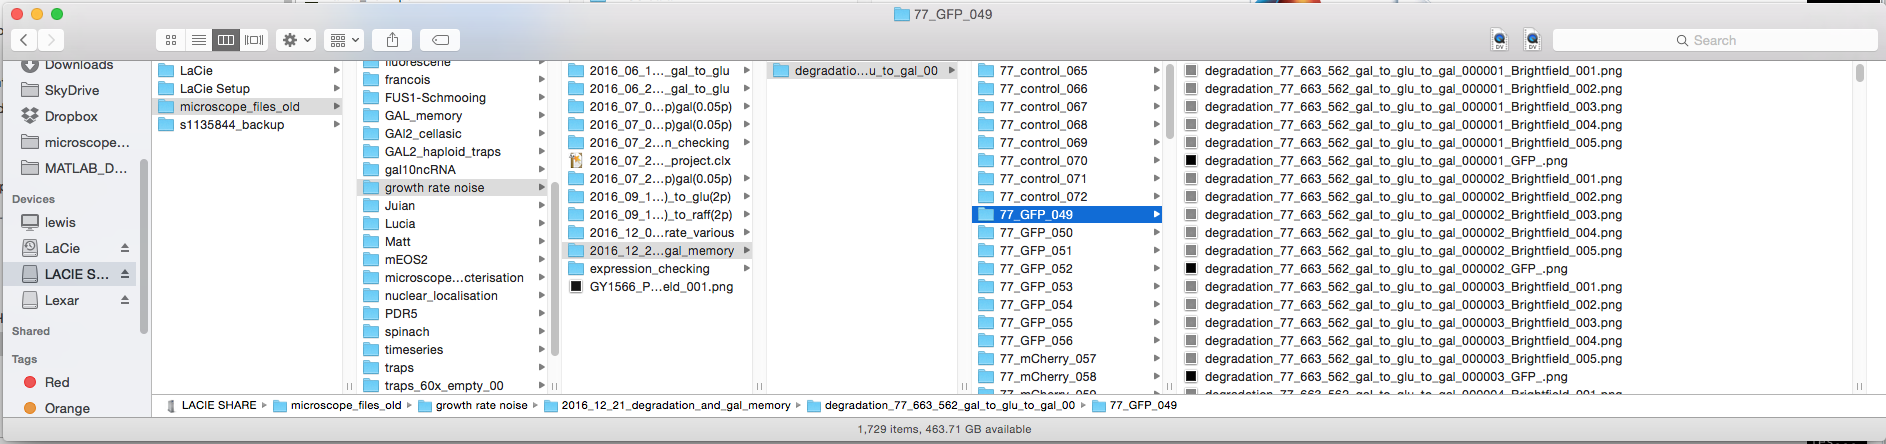
\includegraphics[width=1\linewidth]{documentation_images/other_systems-swain_file_structure}
	\caption[swain lab image file system]{An example of how images are stored in the swain lab image file system. The example shows and experiment called \texttt{degradation\_77\_663\_562\_gal\_to\_glu\_to\_gal\_00} in which Brightfield was imaged with 5 z slices and GFP was imaged with only 1. }
	\label{fig:other_systems-swain_file_structure}
\end{figure}
In order to be able to process the images in anyway, DISCO must of course be able to load your files and therefore know where they are.\\
The DISCO software was designed to be used with files generated by the swain lab microscope control software, which stores files in the form:
\begin{verbatim}
[experiment name]_[6 character timepoint]_[channel name]_[3 character z-slice].png
\end{verbatim}
with each position being stored in a separate folder. An example is shown in figure \ref{fig:other_systems-swain_file_structure}. This is (I believe) also the convention followed by MicroManager. If you're files are arranged in a different structure an you wish to make the software work, there are two options open to you.

\subsubsection{Easy Option: Export Images using ImageJ}
\begin{figure}
\centering
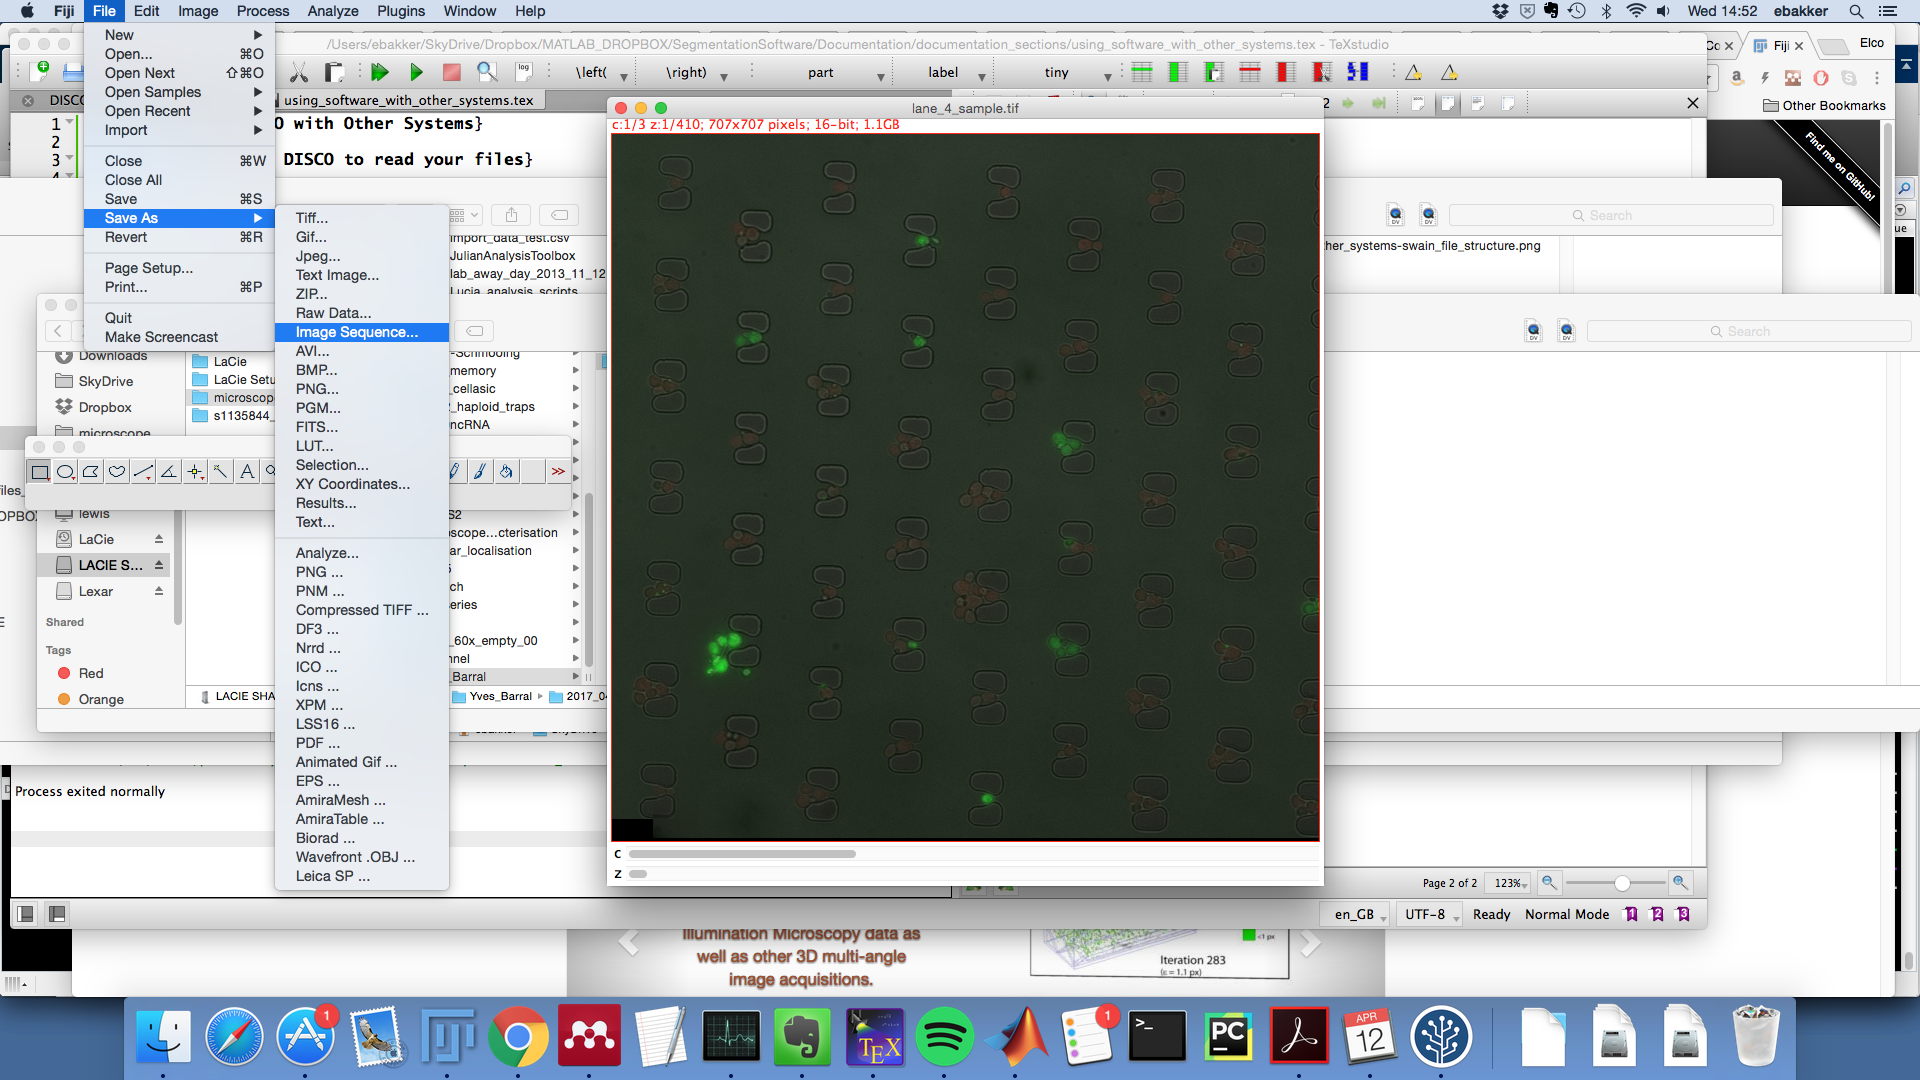
\includegraphics[width=1\linewidth]{documentation_images/other_systems-exporting_from_FIJI}
\caption[Exporting images for processing from FIJI]{Exporting images for processing from FIJI. Shown is the `save' options that should be selected for exporting an image stack for processing from FIJI. Selecting this option will open a dialogue box in which `format' should be set to PNG and `digits' should be set to 6.}
\label{fig:other_systems-exporting_from_FIJI}
\end{figure}


The easiest option is to use ImageJ or \href{https://fiji.sc/}{FIJI} to save your images in this format. These programs can handle most image formats and file structures.\\
First load in an images stack in a way you are happy with. Then save the image stack as an image sequence, choosing a format of PNG and Digits as 6. This will store the image sequence in format appropriate for the software, with channel names given as \texttt{c000001,c000002,c000003 ...}\\
If multiple image stacks are to be processed they can be saved to separate folders in the same parent folder (in imitation of the Swain Lab file structure), allowing the software to be conveniently run on all of them.

\subsubsection{Developer Option: Modify \texttt{timelapseTraps} Constructor and \texttt{timelapseTraps.addChannelsTimelapse} method.}
\newpage
\section{Using DISCO with Later Versions of Matlab}
\label{sec:other_matlabs}

The core of the cell identification software uses the \href{https://github.com/cjlin1/libsvm}{libsvm} library to train and apply linear SVM for pixel classification. The mex files for this are provided, pre-compiled with the software. \\
Unfortunately the original files that were compiled to create these mex files have been lost, and the libsvm library has moved on such that the function calls have changed. Further, later versions of matlab do not seem to necessarily be able to use mex files compiled by older versions. For this reason, matlab versions beyond 2015b will not be able to use the software without some recoding and retraining.\\
This has not yet been undertaken, partly due to laziness and partly because recoding the training and classification is a good opportunity to take a serious look at whether some other classifier (random forest, neural networks etc.) wouldn't provide a better result. \\
When it comes time to retrain, the two parts of the code that will have to be altered are:\\ \texttt{cellVision.classifyImage2Stage}\\
 and the various \texttt{cellVision} methods called in \texttt{ CellVisionTrainingScript.m}:
 \begin{itemize} 
 \item \texttt{generateTrainingSetTimelapseCellEdge}
 \item \texttt{trainSVMCellToOuterLinear} 
 \item \texttt{trainSVMInnerToEdgeLinear} 
\end{itemize}
This is probably all best done by creating a new subclass of \texttt{cellVision}, but I leave such structural decisions to the inheritor.
\vspace*{1cm}
\\This obviously all goes pretty deep into the code, and as such I recommend liasing with current members of the swain lab, or the other author Matt Crane, when undertaking this.
\newpage
\section{Using DISCO when there are no traps}
\label{sec:no_traps}

It should be possible to use DISCO when there are no traps present (such as slides, matec dishes or the cellasic device), but since this is rarely used in the lab it is likely to be a little buggy. \\
To do this the procedure is the same. You \textbf{can} use a cellVision and cellMorphology model trained for cells in traps with good results (provided the imaging modality is similar), but there are one or two in the standard script that cells that shouldn't be run and one or two that should be run even though they seem nonsensical given that you have no traps, so read the comments carefully.\\
If processing slides at single time points (i.e. not timelapses but collections of single timepoints such as for fixed cells) then there is a special GUI (\texttt{experimentTrackingSlidesGUI}) expressly for this purpose. The underlying software and procedure is the same but everything can be done via the buttons (so no need to use the script) and the GUI's are a little better suited to single slides. Note, this GUI is rarely used in the swain lab so may be a bit buggy.



 \bibliographystyle{apalike}
 \bibliography{./library.bib}

%
\end{document}


